\begin{adjustbox}{width=\textwidth}
	\begin{tikzpicture}[every node/.style={inner sep=0,outer sep=0}]
	
		\node [anchor=north east] (imgSpalten) at (-0.03\textwidth,0) {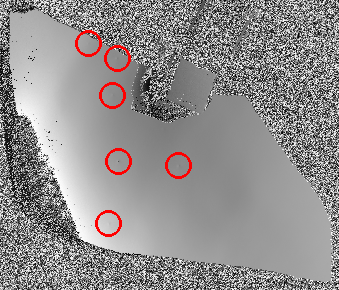
\includegraphics[width=.47\textwidth]{04_deflektometrischeRegistrierung/auswertungDeflektometrischeRegistrierung/figures/pickelDeflektometrischeRegistrierung}};
		\node [below=0.2cm of imgSpalten] {Graubild der Spaltenzuordnung \acrshort{frx}$(x,y)$};
		\node [anchor=north west] (imgGradienten) at (0.03\textwidth,0) {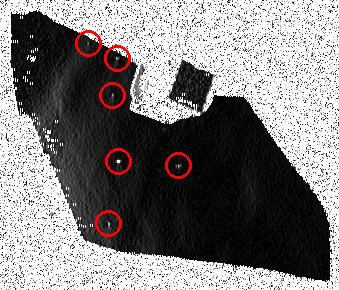
\includegraphics[width=.47\textwidth]{04_deflektometrischeRegistrierung/auswertungDeflektometrischeRegistrierung/figures/pickelGradientenbild}};
		\node [below=0.2cm of imgGradienten, align = center] {Bild der Ableitung von \acrshort{frx}$(x,y)$ \\ in $x$-Richtung};
		
	\end{tikzpicture}
\end{adjustbox}
\caption[Hervorhebung von Pickeln auf reflektierenden Oberflächen.]{Deflektometrische Spaltenregistrierung eines spiegelnden Porzellanbruch\-stücks und das zugehörige Bild der Ableitung. In den rot markierten Stellen lassen sich kleine Abweichungen von einem stetigen Grauwertverlauf erkennen, die in der Ableitung einen Ausschlag haben. Auf dem Prüfobjekt befinden sich an den Stellen kleine Pickel auf der Oberfläche.}